\FloatBarrier
\section{Chapter Summary}
In this chapter, \textit{in-vivo} SFLIM images of anaesthetised rat retinas are recorded using the SFLIO device and the relative concentration of retinal fluorophores are extracted - demonstrating the SFLIM unmixing technique described in the previous chapter. The systemic oxygen consumption of the rat was varied, between \qty{21}{\percent}\ce{FiO2} and \qty{12}{\percent}\ce{FiO2}, to engineer a change in concentration of the fluorescence metabolic marker - FAD. A simplified model of FAD production is derived and is compared to the measured FAD concentration. While a clear image of the retina could not be formed on the SPAD - which would show key features such as the retinal vasculature - the concentration of retinal fluorophores are considered across the whole of the retina. Trends are then established between hypoxia and the concentration of FAD and the statistical significance of these changes is estimated using paired Students t-test and found to be inconclusive and inconsistent across multiple rats. Finally, Principle Components Analysis and Spectral Angle Maps are used to determine if there is a meaningful and detectable change in the fluorescence emission spectra 
\FloatBarrier
\section{FAD as a marker for metabolic health in the retina}\label{sec:FADderivation}
Mapping the concentration of FAD could enable the diagnosis of retinal disease before physical damage to eyesight develops, at the early stage of metabolic dysfunction. FAD is a flavoprotein produced in the body as a by-product of oxygen metabolisation from aerobic respiration (\cref{eq:resp})~\cite{berg2007biochemistry} to create Adenosine Triphosphate (ATP) - the bodies' source of energy:
\begin{equation}\label{eq:resp}
    \ce{C6H12O6 + 6O2 -> 6CO2 + 6H2O + ATP}.
\end{equation}
In the formation of retinal disease, the retina exhibits abnormal metabolic activity - ATP usage - and would present in the retina as areas with abnormal FAD distribution
While the magnitude of the changes in retinal FAD distribution associated with retinal disease is not known, attempts can be made to detect the presence of FAD and assess it feasibility as a diagnostic tool. Changes in FAD concentration can be induced in anaesthetised animal models by artificially restricting systemic oxygen consumption presenting as a detectable change in the SFLIM measurements. In normoxic conditions, \qty{21}{\percent}\ce{FiO2}, oxygen metabolism is typical however in hypoxic conditions ,\qty{15}{\percent}\ce{FiO2}, the retina is starved of oxygen thus lowering the concentration of FAD.
After death - when all metabolic processes have ceased - the systemic concentration should decay to zero - in rat cortices it has been observed that oxygen diffuses from arteries into the surrounding tissue to maintain metabolic activity. This presents as an increase in FAD fluorescence in the tissues. Pictured in \cref{fig:fadhalos} - hyper-fluorescent `halos' of FAD surround arteries and veins~\cite{martinez2017understanding}. 
\begin{figure}[htp]
    \centering
    \includegraphics[width=0.9\textwidth]{figures/ratUCL/FADhaloFigure.pdf}
    \caption{Both (a) and (b) show examples of fluorescence images recorded rat cortices after a short period of acute hypoxia, exhibiting characteristic `halos' of hyper-fluorescent FAD surrounding the vasculature. Increased FAD fluorescence is is attributed to diffusion of arterial and venous oxygen into the retina to maintain metabolic function. Reproduced from Figure 3A and 3B from \citeauthor{martinez2017understanding}\cite{martinez2017understanding}.}
    \label{fig:fadhalos}
\end{figure}
In this chapter, the SFLIO device (described in~\cref{chap:fliodevice}) was used to record \textit{in-vivo} SFLIM images of the retinas of anaesthetised rats under normoxic, hypoxic, and post-mortem conditions where the concentration of retinal FAD is recovered using the SFLIM unmixing algorithm (described in \cref{chap:tensSFLIM}). Successful detection of FAD would be signified by measuring a change in the recovered retinal FAD concentration being compatible with what is expected from changes in FAD produced modelled from aerobic respiration. Another imapactful output could be reproducing the `halo' effect, shown in (\cref{fig:fadhalos}, in the retina. Finally, from this a feasibility of quantifying retinal FAD in human retinas can be explored.
\FloatBarrier
\subsection{\textit{In-vitro} and \textit{Ex-vivo} Studies of Retinal FAD}
Graduating from the simulations presented in \cref{chap:tensSFLIM} to \textit{in-vivo} experiments represents a large, and risk-laden, conceptual jump. Two experiments were performed with limited success to mitigate these risks and gain understanding of the ability of the SFLIO device and SFLIN unmixing technique in detecting changes in FAD at similar concentrations similar to the an \textit{in-vivo} retina. The COVID pandemic limited access to rats for the imaging experiments and due to time constraints these ``failed'' experiments could not be repeated until success. However, for the purpose of demonstrating scientific rigour, and responsible use of animal models, they are briefly described with critiques and suggestions of what could be improved for future experimentation.
\subsubsection{\textit{In-vitro} Resolution of FAD in a Phantom Eye}
In the first of these experiments, three glass capillary tubes were filled with aqueous solutions of FAD, Fluorescein, and Rose Bengal. The solution of FAD was made up to a concentration of 10 times larger than what was estimated to be in the retina (this is discussed in the next section). If FAD would be detectable then, this \textit{In-Vitro} experiment could then be repeated with successively lower concentrations until FAD could no longer be distinguished from Fluorescein and Rose Bengal to give an estimation of the sensitivity of the SFLIO device and SFLIM unmixing analysis to changes in biosimilar concentrations of retinal FAD.
An unfortunate oversight in the experimental design meant that it was only at the analysis stage that the fluorescence lifetime of Rose Bengal was confirmed to be $\approx\qtyrange{750}{800}{\ps}$\cite{jo2005ultrafast} and poor fluorescence efficiency in the excitation range of the SFLIO device (\qtyrange{460}{467}{\nm})\cite{rauf2009solvatochromic}. This then compromises the ability to accurately recover the concentration of each fluorophore since Rose Bengal could not be excited and its lifetime cannot be resolved with the FLIMera.
\textcolor{red}{Insert Figure here and some results from a jupyter notebook}
To significantly improve this experiment for the future, samples of the chemicals AGE and A2E could have been used, and used in aqueous solutions with biosimilar concentrations. This would allow more direct comparisons to the results in \cref{chap:tensSFLIM} and give a more accurate estimations of the systems sensitivity to changes in FAD concentration.

\subsubsection{Imaging of Perfused FAD in \textit{Ex-vivo} Rabbit Models}
The second unsuccessful experiment to discuss applies the techniques in Fluorescein Angiography to measure the effective quantum efficient of fluorescence in the retina to be measured by perfusing an aqueous fluorescein solution through the ophthalmic artery of a post-mortem rabbit and recording FLIM images using a \qty{500}{\nm} long-pass emission filter.
To perfuse dye into the retinal vasculature, a recently sacrificed rabbit (used for cardiac research) had its anterior carotid artery cannulated and, for convenience, the head was removed. The anterior carotid supplies blood to the ophthalmic artery through the Circle-of-Willis~\cite{vrselja2014function} and so by perfusing a dye through this cannula would allow an exogenous dye to be introduced into the retina and imaged.
Time-lapse FLIM and fluorescence intensity images were recorded in parallel as the FAD solution was perfused through the retina. Unfortunately due to malfunctions of the FLIMera, there were no useable FLIM images on the three separate occasions this experiment was attempted. However, as shown in Fig XX, the sCMOS detector was able to record images at multiple time points until the detector saturated.\\
\textcolor{red}{Figure here}
Again, the COVID pandemic compressed the time schedule for experimental work. This meant the perfusion experiment could not be repeated using FAD which could have provided significant insights into how much signal FAD contributes to autofluorescence in the retina. Additionally, this could be used to estimate how the fluorescence emission spectra and the fluorescence lifetime of FAD is affected by scattering and by retinal vasculature and contamination from absorption due to blood, and fluorescence from the eye's lens.
The two experiments described in this section, had they been successful, would have given high confidence in the ability of the SFLIO system to record high-quality images using both the FLIMera and sCMOS detector and also appraise the biochemical resolving power of the system and SFLIM unmxing technique.
\FloatBarrier
\subsection{Estimating The Change in Retinal FAD Concentration at Hypoxia}
The expected variation in FAD concentration as a response to changing oxygenation can be modelled by estimating the rate of FAD production due to oxygen metabolisation in the retina at both normoxia, and hypoxia.\\
The volumetric rate at which oxygen is consumed - better termed as the rate at which blood is deoxygenated - is metabolised, $Q_{\ce{O2}}$, is calculated from the average rate of blood flow through the ophthalmic artery, $Q_{ret}$, and the relative change in saturation of blood entering, ${S\ce{O2}}_{in}$, and exiting, ${S\ce{O2}}_{out}$, it:
\begin{equation}\label{eq:O2rate}
    Q_{\ce{O2}} = Q_{ret}({S\ce{O2}}_{in}-{S\ce{O2}}_{out})H\,,
\end{equation}
The rate of blood flow through the ophthalmic artery was taken as $Q_{ret} = \qty{41.35}{\micro\litre\per\minute}$ by averaging two reported measurements in literature~\cite{dai2013absolute,riva1985blood}. The oxygen saturation - the ratio of oxygenation to deoxygenated haemoglobin in the blood - has been reported as \qty{92.20}{\percent} and \qty{55.60}{\percent} for blood entering and exiting the ophthalmic artery~\cite{dunn2016physiology}. Using~\cref{eq:O2rate} the rate of oxygen metabolisation was estimated to be $Q_{\ce{O2}}=\qty{3.155}{\micro\litre\per\minute}$ where $H=\num{0.2085}$ is H{\"u}ffners constant - the volumetric ratio of oxygen to haemoglobin in the blood~\cite{dunn2016physiology}. Although oxygen is bound to haemoglobin in blood, this value of $Q_{\ce{O2}}$ is expressed in terms of the volume of unbound oxygen at standard temperatures and pressures - volumetric rates of oxygen will be referred to in this way, herein.
The rate of FAD production, $Q_{FAD}$, can then be determined:
\begin{equation}
    Q_{FAD} = Q_{\ce{O2}}k_{FAD}\eta_{FAD}\,,
\end{equation}
where every metabolised \ce{O2} molecule produces $k_{FAD} = 3$ molecules of FAD with an efficiency of $\eta_{FAD} = \qty{1.3}{\percent}$~\cite{berg2007biochemistry,ames1992energy}.
This yields a production rate of $Q_{FAD} = \qty{0.123}{\micro\litre\per\min}$ which is then converted to a steady state volume of FAD by assuming that all FAD in the retina is produced in the time taken for blood to flow through the retina and any FAD, that is consumed, is replaced upon the next circulation period of the heart. With a blood flow period of $\delta T = \qty{4.7}{\second}\equiv \qty{0.078}{\minute}$ measured as the time interval between blood entering and exiting the ophthalmic artery~\cite{khoobehi1990measurement}.
The volume of retinal FAD is then,$V_{FAD} = \qty{9.639}{\nano\litre}$ using:
\begin{equation}
    V_{FAD} = Q_{FAD}\delta T\,.
\end{equation}
which corresponds to $N_{FAD} = \qty{12.27}{\nano\mole}$ using~\cref{eq:nummoles} with a $gfm_{FAD} = \qty{785.56}{\gram\per\mole}$, a density equal to that of water of $\rho_{FAD} = \qty{1}{\gram\per\milli\litre}$, and $N_{A} = \qty{6.022e23}{\per\mole}$.
\begin{equation}\label{eq:nummoles}
    N_{FAD} = V_{FAD}\rho_{FAD}gfm_{FAD}\,,
\end{equation}
Finally, the result of~\cref{eq:nummoles} is expressed as a concentration by approximating the retina as a cuboid with thickness of \qty{344}{\um} and surface area of \qty{1361}{\milli\metre\squared} to estimate its volume~\cite{nagra2017determination,myers2015retinal}:
\begin{equation}\label{eq:FADconc}
    C_{FAD} = \frac{N_{FAD}}{V_{ret}} = \qty{26.9921}{\micro\mole\per\litre}\,,
\end{equation}
In~\citeauthor{batey1991analysis}\cite{batey1991analysis}, the concentration is defined as \qty{39.3}{\pico\mole\per\milli\gram} by weight of the retina which is within \qty{10}{\percent} of the estimation above when converted to equivalent units - $C_{FAD} = \qty{37.64}{\pico\mole\per\milli\gram}$ obtained using the result of \cref{eq:nummoles} and taking the mass of the retina as \qty{326}{\milli\gram}~\cite{batey1991analysis,feke1989blood}. While this analysis does represent a simplified interpretation of the biological functions in the retina it is commensurate with reported measurements of flavoproteins in rabbit eye's. 
\\
The volume of FAD in the retina at hypoxia can then be estimated by assuming that the drop in maximal oxygen consumption, ${\dot{V}\ce{O2}}_{max}$, due to hypoxia will induce a decrease in the volume of retinal FAD of an equal order. This rate of maximal oxygen consumption was measured of sedentary and endurance trained subjects as reported in~\citeauthor{ferretti1997decrease}\cite{ferretti1997decrease} and shown in~\cref{tab:VO2max}. 

\begin{table}[htb]
    \centering
    \begin{tabular}{|c|c|c|}
    \hline
    \ce{FiO2} & \multicolumn{2}{c|}{${\dot{V}\ce{O2}}_{max}$ (\si{\litre\per\minute})}\\
    \cline{2-3}
    & Sedentary & Athletic\\
    \hline
    \qty{21}{\percent} & \num{3.13} & \num{4.11}\\
    \qty{13}{\percent} & \num{2.27} & \num{2.92}\\
    \hline
    \end{tabular}
    \caption{In \citeauthor{ferretti1997decrease}\cite{ferretti1997decrease}, the maximal rate of oxygen consumption was measured of sedentary subjects and subject with a background in endurance sports for a range of inspired oxygen concentrations (\ce{FiO2}). Transcribed from Table.~1 of \citeauthor{ferretti1997decrease}\cite{ferretti1997decrease}.}
    \label{tab:VO2max}
\end{table}
The ratio between the hypoxic and normoxic measurements of ${\dot{V}\ce{O2}}_{max}$ are then $\Gamma = \num{0.725}$, and $\Gamma = \num{0.710}$ for sedentary and athletic subjects, respectively. Taking the case of a sedentary subject the volume of FAD at hypoxia is $V_{FAD,hypoxia} = \Gamma V_{FAD, normoxia} = \qty{6.839}{\micro\litre}$ and the concentration of FAD at hypoxia is estimated as $C_{FAD,hypoxia} = \Gamma C_{FAD, normoxia} = \qty{19.164}{\micro\mole\per\litre}$. \\
In the SFLIM measurements of anaesthetised, hypoxic, rats, the relative mean concentration of FAD it would be expected to be on-the-order of \qty{30}{\percent} lower than the recorded FAD concentration measured of normoxic rats. Although measurements of the concentration of retinal FAD, nor measurements of oxygen saturation in the for hypoxia and normoxic retinas have not been reported for rats this analysis is still useful for confirming that FAD concentration would be expected to decrease under acute hypoxia (\ce{FiO2}) \qty{15}{\percent}. In humans, the decrease of oxygen saturation in the retina, due to acute hypoxia, was reported by \citeauthor{choudhary2013assessment}\cite{choudhary2013assessment}, as \qty{8.2}{\percent} and \qty{8.3}{\percent} for arterial and venous blood, respectively. From this, it could be concluded that a decrease in retinal FAD of $\approx\qty{8}{\percent}$ would be expected due to acute or severe hypoxia. However, as a result of mild hypoxia in humans, the retinal blood vessels dilate by a factor of between \qtyrange{3.5}{21}{\percent}\cite{choudhary2013assessment,frayser1971response} and according to Poiseuille's Law (\cref{eq:poislaw})~\cite{westerhof2019law}:
\begin{equation}\label{eq:poislaw}
    \Delta P \propto  \frac{Q}{r^{4}}\,,
\end{equation}
where the rate of blood flow, $Q$, increases with the fourth-power with an increasing radius of blood vessel, $r$, assuming equal blood pressure, $\Delta P$. 
The change in blood vessel diameter in severe hypoxia, in rats, is not known, which implies that this derived value for FAD concentration is inexact.
% For the above dilation factors this would represent an increase in venous blood flow of~\qtyrange{16}{114}{\percent}. The affect of increased venous blood flow could imply the concentration of retinal FAD would paradoxically increase as a result of acute hypoxia.
This underpins the need for quantitative measurements of retinal fluorophores such as those carried out and presented in this chapter.
\FloatBarrier
\section{\textit{In-Vivo} SFLIM Measurements \\ of Anaesthetised Rats}
SFLIM images of anaesthetised rats, at normixoic and under acuter hypoxia, are recored using the SFLIO device and the concentrations of the fluorophores, AGE, A2E, and FAD, are quantified using the SFLIM unmixing technique. Inducing acute hypoxia will reduce the consumption of oxygen in the retina resulting in a complimentary reduction in the recovered concentration of retinal FAD. If the changes in the measured FAD concentration follow the trend in oxygen consumption then it can be confidently said that FAD was detected and quantified.
\subsection{Experimental Protocol}
Imaging experiments were carried out in the labs of Prof. Kenneth J. Smith (Institute of Neuroinflammation, UCL) where Helen Yang (Institute of Neuroinflammation, UCL) prepared the rats for imaging, administered isoflurane to anaesthetise them, and monitored health throughout the imaging session. An external nitrogen supply was mixed with room-air and fed into a fitted nose-cone to control the fraction of inspired oxygen between \qtyrange{12}{21}{\percent}\ce{FiO2}. Albino rats were chosen for their lack of melanin in the eye which improves the efficiency of excitation, and transmission, of retinal autofluorescence - maximising SNR in detected fluorescence. As shown in~\cref{fig:ratsetup}, the rat is secured to the imaging platform and the pupil is dilated using Tropicamide drops to increase pupil diameter (\qtyrange{1.20}{4.35}{\mm}~\cite{himmel2019pupillary}) - maximising the number of detected photons.


\begin{figure}[htp]
    \centering
    \begin{annotatedFigure}{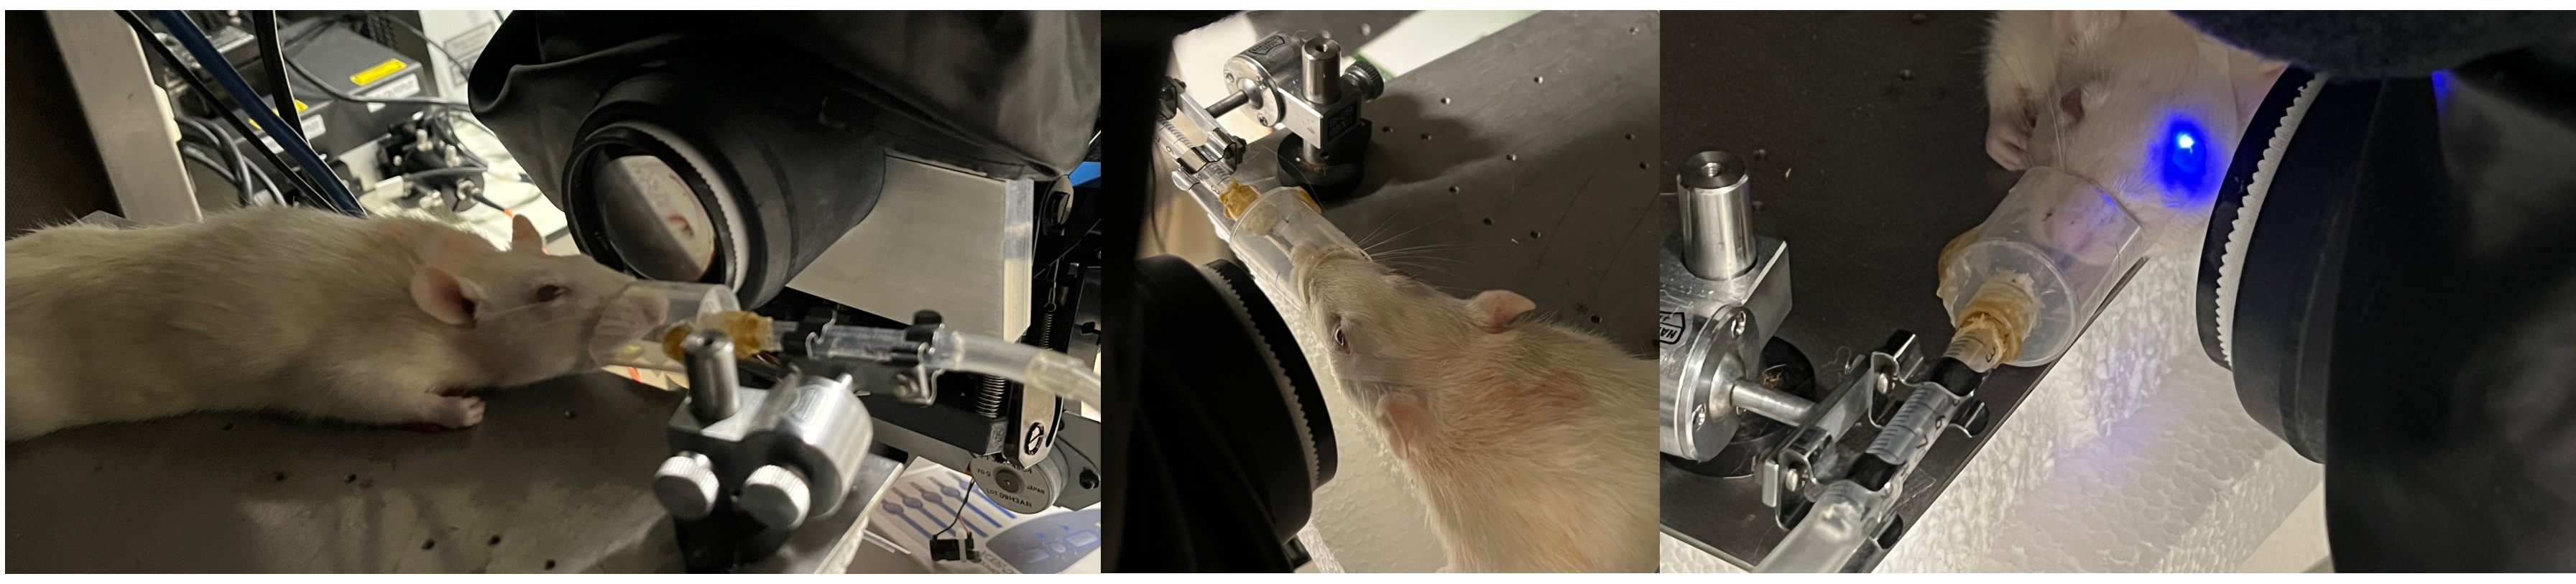
\includegraphics[width = \textwidth]{figures/ratUCL/RatSetupFigure.pdf}}
        \annotatedFigureText{0.015,0.83}{white}{0.3}{a)}
        \annotatedFigureText{0.435,0.83}{white}{0.3}{b)}
        \annotatedFigureText{0.66,0.83}{white}{0.3}{c)}
    \end{annotatedFigure}
    
    \caption{a) and b) The anaesthetised rat is positioned on the imaging platform perpendicular to the SFLIO system to have the rat's retina parallel with the image plane. The fundus camera is moved axially such that the illumination forms a focussed spot on the cornea - evenly illuminating the retina (c).}
    \label{fig:ratsetup}
\end{figure}

Before the retina was imaged, the eyelid is fixed open with stitches and a contact lens is fitted to index-match to the lens of the rats eye. Viscotears gel is applied around the cornea to prevent the eye becoming dry and irritated - inducing additional eye movement and motion requiring correction. To accommodate the rats smaller eyeball diameter, of \qty{6.3}{\mm}~\cite{pazos2015rat}, a field-lens ($\text{diameter} = \qty{50}{\mm}$, $f = \qty{85}{\mm}$) is fitted to the objective lens of the SFLIO device. This additional lens did induce reflections from the illumination source off the front surface of the objective lens and rear surface of the field lens degrading some of the brightfield images with glare (\cref{fig:Ratscmosimages}a) with the penalty of reducing the effectiveness of the motion detection process.
\begin{figure}[htp]
    \centering
    \begin{annotatedFigure}{\includegraphics[width = \textwidth]{figures/ratUCL/RatsCMOSfigure.pdf}}
        \annotatedFigureText{0.025,0.91}{white}{0.3}{a)}
        \annotatedFigureText{0.35,0.91}{white}{0.3}{b)}
        \annotatedFigureText{0.68,0.91}{white}{0.3}{c)}
        \annotatedFigureText{0.19,0.425}{white}{0.3}{d)}
        \annotatedFigureText{0.52,0.425}{white}{0.3}{e)}
    \end{annotatedFigure}
    \caption{a - c) Shows example brightfield images recorded of each of the 3 rats imaged. Each frame is recorded over an integration time of \qty{30}{\ms} at a rate of \qty{10}{\Hz} where a small amount of glare is present in the highlighted region of a). In d) and e) a fluorescence intensity image was recorded using a \qty{500}{\nm} long-pass filter over integration times of \qty{1}{\second} and \qty{5}{\second} respectively.}
    \label{fig:Ratscmosimages}
\end{figure}

This glare was observed to be independent of the motion of the retina which would cause errors in the detected motion in the phase-cross correlation process. By multiplying the images by a mask that is zero in the glare-affected areas and unity elsewhere, the effects of glare was satisfactorily mitigated.  Alternatively, the glare could be removed using an image recorded of a non-reflective scene containing only the glare ($I_{dark}$) and linearly subtracting it from an recorded image ($I_{raw}$) to produce a glare-free image: 
\begin{equation}
    I = \alpha I_{raw} - I_{dark}\,.
\end{equation}
In fluorescence images, shown in \cref{fig:Ratscmosimages}d-e, there was no glare observed but there was not sufficient SNR to record co-registration images to compensate for motion of the retina.
Two rats were imaged over three days - the first rat was imaged on day 1 and day 3, and the second rat was imaged on day 2. For each acquisition, brightfield images are recorded continuously (\qty{50}{\ms} exposure at \qty{10}{\Hz}) in tandem with the FLIMera operating in raw mode over a two minute acquisition period for all 5 spectral filters. Due to the large file size generated from the FLIMera RAW acquisition around \qty{10}{\minute} is required the build and save the \qty{50}{\giga\byte} stream of photon counts for each spectral channel. This SFLIM acquisition is carried out while the rats are cycled from normoxia to hypoxia (\qty{15}{\percent}\ce{FiO2}) and then back to normoxia again with an $\approx 5$~minute interval between each acquisition. These intervals between spectral filters and oxygenation states minimise any photobleaching and should ensure that metabolic processes and FAD concentration re-stabilise although long periods of hypoxia can cause the rat to die due to oxidative stress. SFLIM images were recorded for the first rat on the second day. As described in~\cref{fig:flimerascmossync} the two detectors are synchronised by detecting the Heaviside-like change in photon flux caused by having the laser shutter closed at the start of the acquisition and then opening it a few seconds after. Due to the anaesthetic the nervous response in the rats is suppressed which eliminates any visible saccades in the image sequence. The motion correction algorithm developed in~\cref{chap:motionreg} is still utilised to ensure any small movements of the rat over the hour long imaging sessions does not cause misalignment between spectral filters. However, due to issues in recording a high quality image of the retina on the FLIMera, as will be discussed in \cref{subsec:noFLIMage}, the pixel super-sampling process described in \cref{sec:motionreg} was not carried out.
\FloatBarrier
\subsection{Detected Translational Motion in Rat Retinas}
As discussed in \cref{chap:motionreg}, compensation of retinal motion is required to remove blur in retinal images to produce a high-contrast image where the vasculature is sharply defined. This means the fluorescence decay histograms can be well registered over each spectral band. This would enable any variation in the distribution of FAD in the retina to be resolved with high confidence. Retinal motion is detected from image sequences by computing the phase-cross correlation between a reference image and each successive frame in the sequence - where this reference image is the first fully illuminated frame in the sequence after the laser shutter has been opened. This process was carried out for each spectral channel in the SFLIM acquisition and it was found a simple model of translational motion was sufficient for producing a brightfield image, comprised of motion-corrected frames averaged together. As shown in,~\cref{fig:ratMotionCorrection} this results in higher contrast in the retinal vasculature when compared to an images without correction of motion. 
\begin{figure}[htp]
    \centering
    \begin{annotatedFigure}{\includegraphics[width=0.9\textwidth]{figures/ratUCL/brightfieldRegFigure.pdf}}
        \annotatedFigureText{0.03, 0.82}{white}{0.3}{a)}
        \annotatedFigureText{0.53, 0.82}{white}{0.3}{b)}
    \end{annotatedFigure}
    \caption{Applying the motion compensation algorithm to the brightfield images results in reduced image blur and higher vessel contrast. Approximately 250 raw frames are averaged (a) and motion compensation is applied to each constituent frame and averaged to produce a single corrected frame in (b). For both images the same intensity thresholds, and region-of-interest have been applied.}
    \label{fig:ratMotionCorrection}
\end{figure}
However, in one instance the rat exhibited laboured breathing causing motion that was not just horizontal and vertical translations (see the video sequence titled ``DGeddesPhD\_RatBreatingMotion.mp4''). The differences in image magnification or rotation were small enough in amplitude and frequency that motion can be adequately corrected and characterised using the previously described method in~\cref{chap:motionreg}. 
From~\cref{fig:ratbreathcorrection}, the frequency of the breathing motion was estimated from the time between local minima in the detected translational shifts and was found to be \qtyrange{1}{1.2}{\hertz} corresponding to a heart rate of \numrange{60}{72} beats-per-minute. 

\begin{figure}[htp]
    \centering
    \includegraphics[width = 0.9\linewidth]{figures/ratUCL/RatMotionFigure.pdf}
    \caption{Montage of brightfield image sequence recorded at normoxia after the rat had previously been acutely hypoxia (\qty{12}{\percent}\ce{FiO2}) for a period. Laboured breathing in the rat caused artefacts in the sequence as show above. This is better resolved by viewing the supplementary video ``DGeddesPhD\_RatBreatingMotion.mp4''. This motion is correctable using the existing motion correction algorithm discussed elsewhere \cref{fig:ratbreathcorrection}}
    \label{fig:ratbreathmotion}
\end{figure}


This motion also does not manifest as artefacts or reduced contrast in retinal vasculature within the image as can be seen in \cref{fig:ratbreathcorrection} where an image formed from summing frames over the entire sequence with and without correcting for motion are indistinguishable.

\begin{figure}[htp]
    \centering
    \includegraphics[width=0.9\linewidth]{figures/ratUCL/RatBreathCorrection.pdf}
    \caption{The motion due to laboured breathing does not introduce artefacts in images formed from summing frames over the entire sequence before (left) and after (right) the motion is corrected. These two images are also broadly indistinguishable from a single elemental in the sequence (middle). The translational motion in the X (horizontal) and Y (vertical) directions is plotted (bottom) and shows the periodic nature of the breathing motion.}
    \label{fig:ratbreathcorrection}
\end{figure}
Importantly, the amplitude of the breathing motion is small enough that such at motion with an amplitude of $\approx \num{10}$ pixels on an sCMOS image would manifest as $\approx \num{2}$ pixels on the FLIMera.


\FloatBarrier
\subsection{Addressing Lack of Spatial Variation in SPAD Images}\label{subsec:noFLIMage}
From these imaging experiments, whilst a brightfield image of the retina could be recorded  with sufficient contrast in the blood vessels - a fluorescence image could not be formed on the FLIMera which showed any identifiable retinal features. The exact cause of this is unknown but is worth exploring.
\begin{figure}[htp]
    \centering
    \begin{annotatedFigure}{\includegraphics[width = 0.8\textwidth]{figures/ratUCL/RatUCL-FluorescenceIntensityFigure.pdf}}
            \annotatedFigureText{-0.01,0.92}{black}{0.3}{a)}
            \annotatedFigureText{0.49,0.92}{black}{0.3}{b)}
    \end{annotatedFigure}
    \caption{Fluorescence intensity images recorded of anaesthetised rat retinas recorded with a \qty{500}{\nm} long-pass emission filter using: (a) sCMOS camera with an integration time of \qty{5}{\second}; and (b) the FLIMera with an integration time of \qty{2}{\minute}. For the FLIMera image the fluorescence intensity image is derived by summing photon counts in the time-axis. }
    \label{fig:ratflimcontrast}
\end{figure}

Since both detectors are focussed at infinity, when an image is formed on the sCMOS camera, a complimentary image should be formed on the FLIMera. Before the rats were imaged, a sample of \textit{convallaria majalis} was mounted in the retinal plane of an artificial eye model and brightfield, and fluorescence intensity images were recorded with the sCMOS and FLIMera, respectively. The images were then registered as before in \cref{chap:motionreg} to obtain the affine transform between the detectors - this rules out poor focussing of the camera lenses as the culprit. 
The field lens used to accommodate the smaller, \qtyrange{2}{4}{\mm} diameter pupil of the rat could have caused poor focus in the SPAD image but this is also unlikely since a clear image could be resolved on the sCMOS detector. With the benefit of hindsight, a more rigorous method of evaluating this would be to use a divergent laser source to fill the aperture of the objective lens on the SFLIO device, with the field lens fitted, to ensure that a collimated beam is produced out of lens $f_{1}$. The detectors would then be focused when a focussed spot is produced on the detector - with laser power attenuated so as not to over expose or damage either detector.
Other sources of this lack of spatial variation were also hypothesised but were not experimentally investigated: autofluorescence due to the viscotears used to prevent the cornea drying out; excitation light due to the glare spot bleeding through. The viscotears gel uses the active ingredient, poly-acrylic acid, to prevent drying of the cornea with the sweetener, sorbitol (a sugar alcohol), and sodium hydroxide as preservatives. From an analysis of the available literature: poly-acrylic acid~\cite{xu2019autofluorescence} is not intrinsically fluorescent and only fluoresces when forming hydrogels; sorbitol only emits fluorescence in the near-infrared wavelengths $\lambda >\qty{800}{\nm}$~\cite{lee2019near} which would be blocked by the anti-reflection coatings on the lenses within the SFLIO device; and sodium hydroxide only weakly emits fluorescence between \qtyrange{300}{440}{\nm} when excited at \qty{240}{\nm} and, importantly, only at a hazardous molar concentration of \qty{3}{\mole\per\litre}~\cite{villa2019anomalous} that could not be present in the viscotears gel. Measuring the spectral-temporal fluorescence properties of the viscotears gel would have experimentally demonstrated this. This brief review of the literature does show that the root cause of the inability to produce a focussed image on the FLIMera was not likely to be the viscotears gel.
Reflected excitation light from the field-lens - which produced the glare spot in the brightfield images - could have been insufficiently blocked by the emission filters resulting in $\approx \qty{0.2}{\micro\watt}$ out of the $\approx \qty{2}{\milli\watt}$ excitation source being transmitted through a filter with optical density, $\text{OD} = 4$ which could be sufficiently intense to contaminate the image. However, this is not seen in fluorescence intensity images recorded with the sCMOS detector of the rat retina using the a \qty{500}{\nm} long-pass filter with $\text{OD} = 4$. In this image,~\cref{fig:ratflimcontrast}a, and retinal vasculature were well defined and resolvable unlike an image recorded with the FLIMera where the FLIM image is integrated over time to produce a fluorescence intensity image.
\\
While a high-quality fluorescecne image of the retina, showing key retinal features, could not be recorded with the FLIMera and the root cause could not be ascertained - the SFLIM unmixing algorithm can still be utilised to determined whether we can detect a change in retinal FAD as a response to acute-hypoxia by averaging over the entire retina. This is explored in subsequent sections. 
The contribution of lens fluorescence should next be explored in a pilot experiment using \textit{ex-vivo} rabbit as an analogue for the human eye. An eye could be enucleated shortly after the animal is sacrificed and the retina would be imaged with the SFLIO device as normal. The eyes lens could then be excised and the retinal tissue is then re-imaged. Differences in these two SFLIM datasets would then allow the contamination of the spectra and lifetime, due to the lens, to be appraised.
Finally, an additional pair of SLR lens with higher and lower magnifications could've been trialled to assess how far out-of-focus the FLIMera was despite the convallaria sample being in-focus.
\FloatBarrier
\section{Recovering FAD Concentration Using SFLIM Unmixing}
Although clear fluorescence images of the retina could not be formed on the FLIMera, the concentration of retinal FAD can be estimated over the entire FOV using the previously developed SFLIM unmixing algorithms. The SFLIM unmixing method was applied to SFLIM data with and without the application of motion correction. The relative concentrations of retinal fluorophores for each pixel on the FLIMera and the mean concentration can be calculated after masking out malfunctioning pixels with the pixel mask discussed in~\cref{sec:pixelmask}. The recovered fluorophore concentrations were then compared over the Normoxia, Hypoxia, Normoxia, and in one case~\textit{post-mortem} to establish if the detected changes fitted the predictions made in~\cref{sec:FADderivation}. The statistical significance was calculated using a paired student t-test to establish whether a change in retinal fluorophore concentration was detected as a result of a change in the rats physiology or just due to noise. Finally, Principle Components Analysis (PCA) to assess whether the detected changes are due to changes in the fluorescence emission spectra or the fluorescence lifetime.
\FloatBarrier
\subsection{Darkfield Correction}\label{subsec:darkfield}
In the first two of three imaging sessions the fluorescence decay was contaminated by a dark current which appeared as a Gaussian-like function superimposed onto the fluorescence decay (see \cref{fig:darkfieldGauss}). Darkfield FLIM measurements were recorded with the FLIMera covered and the laser shutter closed, such that any signal recorded would originate from either thermal noise or due to this anomalous dark current. After discussions with the manufacturer of the FLIMera it was confirmed this dark-current was due to poor calibration of the pulse-converter which converts the analogue signal produced by the laser when a pulse is emitted to a digital signal that is at logic-high when photons are to be counted. This was corrected for the final rat imaging session and subsequent fluorescence decays did not exhibit this dark current.
\\
\begin{figure}[htp]
    \centering
    \includegraphics[width=0.9\textwidth]{figures/ratUCL/DarkfieldCorrectionFigure.pdf}
    \caption{The anomally in the fluorescence decays was measured (a) and characterised by aggregating across the whole SPAD and, fitting to 3 appropriate functions: A Gaussian (\cref{eq:gauss}); a  $\text{sec}^{2}h$ curve (\cref{eq:sech}); and the derivative of a sigmoid} (\cref{eq:divsigmoid})
    \label{fig:darkfieldGauss}
\end{figure}
\\
If not accommodated in the unmixing process, this time-dependent dark current would result in poor convergence of minimising-function, $\varphi(\mathbf{x})$:
\begin{equation}\label{eq:lsqminimisiertensor}
    \varphi(\mathbf{x}) = \big\lvert\big\lvert \mathcal{A}\bullet_{3}\mathbf{x} - \mathbf{M}\big\rvert\big\rvert_{F}^{2}\,,
\end{equation}
to a solution, $\mathbf{x}$, given that contamination in the SFLIM measurement, $\mathbf{M}$, is not accounted for in the model of endmember abundances, $\mathcal{A}$. Ultimately this would yield unreliable and biased fluorophore concentrations. Instead, the affected time period could be masked out and this region is excluded when evaluating the minimising function.
Programmatically this is implemented through slicing the $\lambda T$ array containing the result of $\mathbf{\Psi} = \mathcal{A}\bullet_{3}\mathbf{x} - \mathbf{M}$. Mathematically this can be written as excluding time-bins on the intervals $[0, t_{1}]$ and $[t_{2},t_{3}]$:
\begin{align}
        \varphi(\mathbf{x}) &= \big\lvert\big\lvert \mathcal{A}\bullet_{3}\mathbf{x} - \mathbf{M}\big\rvert\big\rvert_{F}^{2} = \big\lvert\big\lvert\mathbf{\Psi}\big\rvert\big\rvert_{F}^{2}\\
        &=\sum_{\lambda}\sum_{T}\lvert\mathbf{\psi_{\lambda t}}\rvert^{2} = \sum_{\lambda}\Bigg(\sum_{0}^{t_{1}}\lvert\mathbf{\psi_{\lambda t}}\rvert^{2} + \sum_{t_{2}}^{t_{3}}\lvert\mathbf{\psi_{\lambda t}}\rvert^{2}\Bigg)
\end{align}
Subsequently, the minimising function, $\varphi(\mathbf{x})$ can be represented as the sum of two separate minimising functions over these intervals such that:
\begin{align}
    \varphi(\mathbf{x}) = \big\lvert\big\lvert\mathbf{\Psi}\big\rvert\big\rvert_{F}^{2}\bigg\rvert_{t=0}^{t=t_{2}} + \big\lvert\big\lvert\mathbf{\Psi}\big\rvert\big\rvert_{F}^{2}\bigg\rvert_{t=t_{2}}^{t=t_{3}}
\end{align}
While the dark-current could be characterised by fitting a Gaussian:
\begin{equation}\label{eq:gauss}
    y(x, A,\mu,\sigma,c) = A\exp(\frac{-(x-\mu)^{2}}{2\sigma^{2}})+c\,,
\end{equation}
(\cref{eq:gauss}) or $\sec^{2}h$:
\begin{equation}\label{eq:sech}
    y(x,x_{0},A,\tau) = A\text{sech}^{2}\bigg(\frac{x - x_{0}}{\tau}\bigg)+c\,,
\end{equation}
or the derivative of a sigmoid function:
\begin{equation}\label{eq:divsigmoid}
    y(x,x_{0}, A, \tau,c) = \dfrac{d}{dx}\frac{1}{1+\exp(-\tau*(x-x_{0}))}\,,
\end{equation}
to each pixel and then subtracting the fitted noise-profile from the affected histogram but this could result in over-fitting in histograms with low photon counts - increasing sensitivity to noise. 
The masking approach, however, trades-off leaving insufficient photons for unmixing when too many time bins are masked and masking too few bins leaves the histogram still contaminated - biasing the recovered flourophore concentrations. A masking window of 30 pixels was selected to strike this balance which left on around \num{1000} photons used in the unmixing process after masking the dark-current and excluding the first $\approx 50$ time-bins to remove the influence of the temporal response of the SFLIO device. This process did result in more instances where the minimiser could not converge to a suitable minima of $\varphi(\mathbf{x})$ which results in a vector of ``NaN''s being returned - which are masked out in the SFLIM unmixing process. 
\\
As an aside, the contaminated time-bins were removed and the remaining photon counts were summed to produce a fluorescence intensity image.
\begin{figure}[htp]
    \centering
    \begin{annotatedFigure}{    \includegraphics[width=0.6\textwidth]{figures/ratUCL/DarkFieldMaskFigure.pdf}}
        \annotatedFigureText{0.04,0.96}{black}{0.3}{a)}
        \annotatedFigureText{0.46,0.96}{black}{0.3}{b)}
    \end{annotatedFigure}
    \caption{When using the fitted Gaussian as a mask to remove the darkfield there is no affect to the structure or spatial variation in the raw SPAD image (a) or the darkfield corrected image (b)}
    \label{fig:masked-unmaskedintensityimage}
\end{figure}
The darkfield-corrected images, \cref{fig:masked-unmaskedintensityimage}b, shows only minimal differences to the SPAD image, \cref{fig:masked-unmaskedintensityimage}a. Thus the issue of SPAD images of the retina having no resolvable details.
\FloatBarrier
\subsection{Trends in Retinal Fluorophore Concentration as a Response to Acute Hypoxia}\label{subsec:meanfluor}
The concentrations of the retinal fluorophores, FAD, AGE, and A2E, can now be estimated from SFLIM measurements with the SFLIM unmixing algorithm and any trends due to changes in oxygenation state can be established. Before this analysis, the SFLIM data is processed to mask malfunctioning pixels, the fluorescence decays are aligned in the time axis, and the time-bins affected by the previously mentioned dark-current are also masked as described in \cref{sec:pixelmask}.
The unmixing algorithm is performed on SFLIM measurements for each functional pixel on the SPAD array to produce images of relative fluorophore concentrations - shown in \cref{fig:rat1session1fluormaps,fig:rat2session1fluormaps,fig:rat1session2fluormaps}. 

\begin{figure}[htp]
    \centering
    %figure for rat1 session 1
    \centering
    \includegraphics[width=0.8\textwidth]{figures/ratUCL/Rat1Session1FlourophoreMaps.pdf}
    \caption{Maps of relative concentration of retinal fluorophores, FAD, AGE, and A2E, recovered from SFLIM measurements recorded of rat 1 in the first imaging session under anaesthesia. The oxygen consumption of the rat is varied between normoxia (\qty{21}{\percent}\ce{FiO2}), hypoxia (\qty{12}{\percent}\ce{FiO2}, and normoxia again (\qty{21}{\percent}\ce{FiO2}) for each SFLIM measurement. In the unmixing process, the constraint that for each XY pixel the concentrations should not be greater than unity.}
    \label{fig:rat1session1fluormaps}
\end{figure}
\begin{figure}[htp]
    % figure for rat2 session 1
    \centering
    \includegraphics[width = 0.8\textwidth]{figures/ratUCL/Rat2Session1FlourophoreMaps.pdf}
    \caption{Maps of relative concentration of retinal fluorophores, FAD, AGE, and A2E, recovered from SFLIM measurements recorded of the rat 2 its first imaging session under anaesthesia. The oxygen consumption of the rat is varied between normoxia (\qty{21}{\percent}\ce{FiO2}), hypoxia (\qty{12}{\percent}\ce{FiO2}, and normoxia again (\qty{21}{\percent}\ce{FiO2}) for each SFLIM measurement. A final SFLIM measurement of the rat was recorded after the rat was sacrificed. In the unmixing process, the constraint that for each XY pixel the concentrations should not be greater than unity.}
    \label{fig:rat2session1fluormaps}
\end{figure}
\begin{figure}[htp]
    \centering
    \includegraphics[width = 0.8\textwidth]{figures/ratUCL/Rat1Session2FlourophoreMaps.pdf}
    \caption{Maps of relative concentration of retinal fluorophores, FAD, AGE, and A2E, recovered from SFLIM measurements recorded of rat 1 in the second imaging session \qty{48}{\hour} after it was first anaesthetized and imaged (see \cref{fig:rat1session1fluormaps}). The oxygen consumption of the rat is varied between normoxia (\qty{21}{\percent}\ce{FiO2}), hypoxia (\qty{12}{\percent}\ce{FiO2}, and normoxia again (\qty{21}{\percent}\ce{FiO2}) for each SFLIM measurement. In the unmixing process, the constraint that for each XY pixel the concentrations should not be greater than unity.}
    \label{fig:rat1session2fluormaps}
\end{figure}
Much like the integrated intensity maps in (\cref{fig:rat1session1fluormaps,fig:rat2session1fluormaps,fig:rat1session2fluormaps}) these maps of fluorophore concentration show no variation across the image that could be correlated to structures in the retina. It would be expected that there would be a background level of FAD due to blood circulating around the choroid and areas of increased FAD around the arteries. 
Trends between the mean retinal fluorophore concentration and changes in oxygenation state can still be established using these unmixed fluorophore maps.
\FloatBarrier
\subsubsection{Trends in Retinal Fluorophore Concentration Related to Changes in Oxygenation State}
For each rat, and each oxygenation state, the mean fluorophore concentration was calculated in terms of the number of photons each fluorophore FAD, AGE, and A2E contributes to the total fluorescence signal. Now the prediction made at the start of this chapter - that FAD concentrations should decrease at acute hypoxia, relative to normoxic condition - can be evaluated. If this holds true, then it can be concluded that it is likely that retinal FAD has been detected.
In \cref{fig:fluorTrendsPhotons}a-c) these mean concentrations are plotted and shows that in all three imaging sessions, the recovered FAD concentration decreased with acute hypoxia. 

\begin{figure}[htp]
    \centering
    \begin{annotatedFigure}{\includegraphics[width=0.99\textwidth]{figures/ratUCL/FluorTrends.pdf}}
        \annotatedFigureText{0.01,0.99}{black}{0.3}{a)}
        \annotatedFigureText{0.51, 0.99}{black}{0.3}{b)}
        \annotatedFigureText{0.22, 0.53}{black}{0.3}{c)}
    \end{annotatedFigure}
    \caption{Trends in recovered retinal fluorophore concentrations as a result of induced changes to systemic oxygenation. Fluorophore concentrations calculated by dividing the \qty{2}{\minute} acquisition period into \num{10} sub-acquisitions of equal length and then expressed in terms of average number of photons per pixel in that sub-acquisition. Error bars are presented as the standard error of the \num{10} sub-acquisitions}
    \label{fig:fluorTrendsPhotons}
\end{figure}

This assertion should not be without scrutiny. Error bars were calculated as the standard error of the mean of repeated measurements of mean retina fluorophore concentrations, constructed from splitting the SFLIM measurements into 10 short sub-acquisitions and recovering retinal fluorophores. As can be seen, most of the reduction in FAD between normoxia and hpyoxia can be attributed to variance in the measurements due to low-photon counts and the possibility of the fluorophores becoming bleached. \\
Additionally, it was predicted that when the rat transitions back to normoxia from hypoxia the FAD concentration should return to its previous levels. This is not seen in the the recovered mean concentrations of FAD. In the one instance where the rat was sacrificed and a SFLIM dataset was acquired the FAD concentration does not decay to zero when all metabolic processes cease. A paired student t-test was then carried out on each pair of change in oxygenation to assess whether the trends in retinal fluorophores is due to a change in the oxygenation of the rat or simple variation in the measurements due to high noise.


\FloatBarrier
\subsection{Assessing Statistical Significance of FAD Response}\label{subsec:ttest}
The error, or variation, in the recovered fluorophore concentrations is on the same order as the change in mean-concentration between oxygenation states. This introduces uncertainty in whether the change in FAD concentration that was measured is actually caused by varying the consumption of oxygenation in the rat or simply, random variation in the measurement. To address this concern a ``Student Paired t-test'' was performed on the recovered fluorophore concentration to bound the probability, $p$, of the change we measured being due to variation in the measurement - termed "null hypothesis" - with the probability that the induction of hypoxia did cause a change in the FAD concentration with probability $1-p$. 
To perform a Student Paired t-test. The standard error of the mean of differences between the recovered concentrations for two oxygenations states, $x_{i}$ and $y_{i}$ is calculated to derive the T-statistic, $T = \nicefrac{\Bar{\Delta}_{xy}}{\Bar{\sigma}_{xy}}$. Where $\Bar{\Delta}_{xy}$ is the mean difference between two oxygenation states, $x$ and $y$, 
\begin{equation}
    \overline{\Delta}_{xy} = \overline{ x_{i} - y_{i}}\,
\end{equation}
and $\overline{\sigma}_{xy}$ is the standard error computed from the standard deviation, $\sigma_{xy}$, over $n$ samples.
\begin{equation}
    \overline{\sigma}_{xy} = \frac{\sigma_{xy}}{\sqrt{n}}
\end{equation}

By comparing the T-statistic with a $t$-distribution:
\begin{equation}\label{eq:tdist}
    f(t) = \frac{\Gamma(\frac{n+1}{2})}{\sqrt{\pi}\Gamma(\frac{n}{2})}\Bigg(1 + \frac{t^{2}}{n}\Bigg)^{-(\frac{n+1}{2})}\,,
\end{equation}
with $n$ degrees-of-freedom, the $p$-value can be extracted to give a probability of the null-hypothesis. 
For each fluorophore the change in concentration is calculated as the percentage change of total number of photons recorded over two different oxygenation states. The $p$-value is then computed using a $t$-distribution look-up table (``\textit{scipy}'' \textit{python} package) and is shown in \cref{tab:ttestMain}. 

\begin{table}
    \begin{subtable}[t]{0.9\textwidth}
    \centering
    \sisetup{table-alignment-mode=format, round-mode=figures, table-column-width=1.5cm}
    \small
    \begin{tabular}{|p{3.2cm}|  S[round-precision=4]|
                                S[round-precision=2]|
                                S[round-precision=4]|
                                S[round-precision=2]|
                                S[round-precision=4]|
                                S[round-precision=2]|
                                S[round-precision=4]|
                                S[round-precision=2]|
                                S[round-precision=4]|
                                S[round-precision=2]|}
        \hline
        & \multicolumn{2}{c|}{Rat 1 - Session 1} & \multicolumn{2}{c|}{Rat 2 - Session 1} & \multicolumn{2}{c|}{Rat 1 - Session 2} \\
        \hline
       Change in Oxy.& {$\Delta_{FAD}$} & {$p$-value}  & {$\Delta_{FAD}$} & {$p$-value}  & {$\Delta_{FAD}$} & {$p$-value} \\
        State & {(\%)} & & {(\%)} & & {(\%)} &\\
       \hline
       Norm. To Hyp. & \num{-31.306511215525244} & \num{4.78989243667469e-07} & \num{-54.83078399530178} & \num{5.535602434791192e-09} & \num{-32.76058614849388} &\num{5.438630613110299e-09}\\
       \hline
       Hyp. To Nor. 2 & \num{7.896276165081215} & \num{0.04001956386363361} & 14.76457257722695 & \num{4.7271147283432893e-07} & \num{51.55500731722816}& \num{2.053319524750847e-06}\\
       \hline
       Norm. To Norm. 2 &  \num{-24.501622691262938} & \num{8.510036758754948e-09} & \num{-43.60961563462101} & \num{2.926951097621746e-08} & \num{22.68463380231996} &\num{2.520271452591082e-04}\\
       \hline
       Norm. To Death & &  &\num{-43.609523917005596}& \num{2.9270614725268114e-08}& &  \\
       \hline
       Hyp. To Death &  &  &\num{14.764680152018073}& \num{4.726990805630476e-07}&  &  \\
       \hline
       Norm. 2 To Death & & & {\num[round-mode=places, round-precision=4]{0.00011}} &\num{0.05743584614696069}& & \\
       \hline
                                
    \end{tabular}
    \caption{t-test results for FAD}
    \label{tab:ttestFAD}
    \vspace*{1cm}
    \end{subtable}
    
    \begin{subtable}[t]{0.9\textwidth}
    \centering
    \sisetup{table-alignment-mode=format, round-mode=figures, table-column-width=1.5cm}
    \small
    \begin{tabular}{|p{3.2cm}|  S[round-precision=4]|
                                S[round-precision=2]|
                                S[round-precision=4]|
                                S[round-precision=2]|
                                S[round-precision=4]|
                                S[round-precision=2]|
                                S[round-precision=4]|
                                S[round-precision=2]|
                                S[round-precision=4]|
                                S[round-precision=2]|}

        \hline
        & \multicolumn{2}{c|}{Rat 1 - Session 1} & \multicolumn{2}{c|}{Rat 2 - Session 1} & \multicolumn{2}{c|}{Rat 1 - Session 2} \\
        \hline
       Change in Oxy.& {$\Delta_{AGE}$} & {$p$-value}  & {$\Delta_{AGE}$} & {$p$-value}  & {$\Delta_{AGE}$} & {$p$-value} \\
        State & {(\%)} & & {(\%)} & & {(\%)} &\\
       \hline
       Norm. To Hyp. & \num{36.73845540879449} & \num{1.2129855908953851e-09} & \num{55.94262439767155} & \num{0.1588847726902607} & \num{-4.869533327623472} &\num{0.01476854947998337}\\
       \hline
       Hyp. To Nor. 2 & \num{-36.47776055506893} & \num{5.458684853053609e-10} & \num{-67.14473694997025} & \num{0.028701101342988936} & \num{-4.58604064439413}& \num{0.03315636788775767}\\
       \hline
       Norm. To Norm. 2 &  \num{0.5207084290772277} & \num{0.378107436641914} & \num{-15.264845593890513} & \num{0.04101290831611819} & \num{-9.376587991622035} &\num{0.004406940283828267}\\
       \hline
       Norm. To Death & &  &\num{-15.264100742018567}& \num{0.005133755889685807}& &  \\
       \hline
       Hyp. To Death &  &  &\num{-67.14432734548367}& \num{3.682486022535063e-08} &  &  \\
       \hline
       Norm. 2 To Death & & & {\num[round-mode=places, round-precision=4]{0.000819894114190679}} &\num{0.032766934545733456}& & \\
       \hline                                
    \end{tabular}   
    \caption{t-test results for AGE}
    \label{tab:ttsetAGE}
    \vspace*{1cm}
    \end{subtable}
    \begin{subtable}[t]{0.9\textwidth}
    \centering
    \small
    \sisetup{table-alignment-mode=format, round-mode=figures, table-column-width=1.5cm}
    \begin{tabular}{|p{3.2cm}|  S[round-precision=4]|
                                S[round-precision=2]|
                                S[round-precision=4]|
                                S[round-precision=2]|
                                S[round-precision=4]|
                                S[round-precision=2]|
                                S[round-precision=4]|
                                S[round-precision=2]|
                                S[round-precision=4]|
                                S[round-precision=2]|}   
        \hline
        & \multicolumn{2}{c|}{Rat 1 - Session 1} & \multicolumn{2}{c|}{Rat 2 - Session 1} & \multicolumn{2}{c|}{Rat 1 - Session 2} \\
        \hline
       Change in Oxy.& {$\Delta_{A2E}$} & {$p$-value}  & {$\Delta_{A2E}$} & {$p$-value}  & {$\Delta_{A2E}$} & {$p$-value} \\
        State & {(\%)} & & {(\%)} & & {(\%)} &\\
       \hline
       Norm. To Hyp. & \num{62.13010322707054} & \num{1.0740993673380998e-11} & \num{5.027149310079019} & \num{0.08183947292419991} & \num{-26.69017034022325} &\num{5.154642206973885e-09}\\
       \hline
       Hyp. To Nor. 2 & \num{-42.71268278804473} & \num{1.830243802194944e-12} & \num{-28.48335445402891} & \num{0.05633120789198803} & \num{6.639735558159754}& \num{3.0127109988835988e-06}\\
       \hline
       Norm. To Norm. 2 &  \num{26.420008804075852} & \num{2.0075775208559094e-07} & \num{-23.65399336336594} & \num{0.07484643982404204} & \num{-20.46661779529254} &\num{3.5187463156723894e-08}\\
       \hline
       Norm. To Death & &  &\num{-23.654034685580303}& \num{5.615975463161401e-05} & &  \\
       \hline
       Hyp. To Death &  &  &\num{-28.483398694681544}& \num{1.3725568075817538e-07} &  &  \\
       \hline
       Norm. 2 To Death & & &{\num[round-mode=places, round-precision=5]{-0.00005589514560848622}} & \num{0.37480529225054726} & & \\
       \hline
    \end{tabular}
    \caption{t-test results for A2E}
    \label{tab:ttestA2E}
\end{subtable}
\caption{The $p$-value for the measured changes in the concentration of the fluorophores FAD, AGE, and A2E has been calculated for each pair of oxygenation states for each imaging session: Normoxia to Hypoxia; Hypoxia back to Normoxia; between the both measurements of a Normoxic state; and permutations where the rat was sacrificed. Lower $p$-values indicate a higher likelihood that a physiological change was detected in the SFLIM measurements - variation in the results is not simply due to sample variation}
\label{tab:ttestMain}
\end{table}
For FAD over all 3 imaging sessions a similar decrease in apparent FAD concentration is recorded with $p$-values indicating a high confidence that ``something'' has changed in response to changing the rats physiology. This follows the expectations set out in the beginning of the chapter but there are some disagreements. Interestingly, what is not seen is the concentration of FAD returning to its initial value after the rat is returned to a normoxic state after being in hypoxia - implying that the FAD is not being restored when after no longer being hypoxic. A disagreement in the recovered FAD concentrations with the expected change due to physiology is also seen in SFLIM measurements from where the rat is sacrificed - all metabolic functions have ceased - and all the FAD in the retina should have dissipated. While the measured concentration of FAD does show a decrease from the initial normoxic state to death (albeit not to zero) the \textit{post-mortem} FAD concentration is the same or higher when the rat is hypoxic, or the same when compared to when the rat is normoxic after having been hypoxic. This is true for all 3 fluorophores when comparing this second normoxic state to \textit{post-mortem} fluorophore concentrations.
This incongruence between the recovered fluorophore concentrations and what was expected from the variations of physiology required further analysis into whether the SFLIM measurements actually show variation between oxygenation states. In the next section, a simple technique of Principle Components Analysis is used on the spectral domain to uncover changes between oxygenation states to motivate the hypothesis that changes in recovered FAD changes are correlated to changes in SFLIM measurements.


\FloatBarrier
\subsection{Comparing Detected Changes with PCA and Spectral Angle Maps}\label{subsec:pcarat}
To reinforce the connection between the recovered FAD concentration and oxygenation state, the technique Principle Components Analysis (PCA) can be used to test two hypotheses: (1) that the SFLIM measurements show changes in the spectra and lifetime domain as a response to changing physiology in the rat; and (2) SFLIM unmixing algorithm is capable of uncovering these changes with sufficient accuracy and precision to detect FAD. PCA uses a coordinate transformation to reduce the number of orthonormal bases (dimensions) in a dataset to those which exhibit the most variation or information. This technique is particularly useful for distilling higher-dimensional datasets into typically 2 dimensions that can be visualised by humans and is readily used for identifying unique endmembers in spectral images~\cite{chang2018review,nascimento2005vertex}. The SFLIM measurements of \textit{in-vivo} rat retinas can be reduced into spectral images, by integrating the SFLIM dataset over time, and analysed using PCA to identify if the fluorescence emission spectra is changing as a response to hypoxia - with premise being that each oxygenation state will occupy unique regions in the plane of 2 principal components.
\subsubsection{PCA Maps of SFLIM Data}
Before the principal components can be used, the SFLIM measurements are formed into spectral images by summing across the time axis of the $I(x,y,t,\lambda)$ volume and area normalised to form $I'(x,y,t,\lambda)$:
\begin{equation}
    I'(x,y,t,\lambda) = \frac{I(x,y,t,\lambda)}{\int_{0}^{\infty}I(x,y,t,\lambda)d\lambda}
\end{equation}
The area normalisation allows for spectra of the same pixel on the SPAD $(XY)$ but differing oxygenation state to be compared. The 4D point-clouds - 1 dimension for each spectral band - for each oxygenation states are then concatenated such that the principal components are optimised for the every oxygenation state. The first two principle components are then found and the corresponding coordinate transformation is applied to produce 2D point-clouds which are colour-coded for each oxygenation state in~\cref{fig:ratPCA}.


\begin{figure}
    \centering
    \begin{annotatedFigure}{\includegraphics[width=0.9\textwidth]{figures/ratUCL/RatOxygenationPCAPlot.pdf}}
        \annotatedFigureText{0.01,0.97}{black}{0.3}{a)}
        \annotatedFigureText{0.53,0.97}{black}{0.3}{b)}
        \annotatedFigureText{0.24,0.50}{black}{0.3}{c)}

    \end{annotatedFigure}
    \caption{First 2 principal components of spectra images recorded of the pair of rats that were imaged over 3 sessions (a-c). The normoxic and hypoxic point clouds occupying separate regions in (a) and (c) indicates that as a response to hypoxia the fluorescence emission of the retina does change. The fact that the other oxygenation states do not form unique clusters does indicate either the restoration of metabolic function after hypoxia takes place over longer than expected time scales and/or a shortcoming in the SFLIM unmixing algorithm and SFLIO device.}
    \label{fig:ratPCA}
\end{figure}
In \cref{fig:ratPCA}a and \cref{fig:ratPCA}c, there are visibly separate regions occupied by the spectra of the normoxic and hypoxic states indicating that there is a change in the fluorescence emission spectra in the rat retina as a response to acute hypoxia. However, what is not evident in \cref{fig:ratPCA}a-c - but was expected - would be significant overlap between the regions of the initial normoxic state and the spectra recorded after the rat was brought back to normoxia after being hypoxic. Instead, it appears that the measurements of the second period of normoxia highly overlap the hypoxic measurements which could be explained as a combination of both physiological factors and a limitation of the SFLIO device and SFLIM unmixing algorithm. When transitioning between oxygenation states the rats were allowed a period of \qtyrange{2}{3}{\minute} to allow metabolic functions to stabilise or return to normal. It is likely that if the period between SFLIM acquisitions was not long enough then this would result in the metabolites such as FAD, and AGE not being fully replenished and being produced at a healthy rate before the next SFLIM dataset was recorded. As to the high overlap between every oxygenation state when the first rat was re-imaged, phototoxic damage to the retina from the long and intense exposure of the previous imaging session could have disrupted the production of metabolites, FAD and AGE, and damaged the RPE which is responsible for the fluorescence of A2E~\cite{crouch2015a2e,rozanowska2023lipofuscin}. The lasers exposure would be estimated to be around $\numrange{2.5}{3}\times$ as intense~\cite{yao2021understanding} as the safety threshold for safe human imaging and sustained for over \qty{30}{\minute} and could readily result in permanent damage to the rats retina.
\FloatBarrier
\subsubsection{Quantifying Changes in Fluorescence Emission Spectra as a Response to Hypoxia}
The perceived separation in the map of principal components in \cref{fig:ratPCA} can be quantified using the metric of the Spectral Angle Map (SAM), 
\begin{equation}\label{eq:sam2}
    \varphi = \frac{\mathbf{a}\cdot \mathbf{b}}{\lvert \mathbf{a} \rvert\,\lvert \mathbf{b} \rvert}\,,
\end{equation}
to calculate the overlap between pairs of spectra pertaining to oxygenation states $\mathbf{a}$ and $\mathbf{b}$ with a range of \numrange{-1}{1}. High correlation between the spectra of two oxygenations states will show a $\varphi$ of \num{0} and spectra with no correlation will be have a $\varphi$ near \num{1} or \num{-1}.\\
Traditionally, the SAM is calculated, using \cref{eq:sam2}, as $\theta = \arccos{(\varphi)}$ and expressed in radians, however, the $arcos$ function is not surjective (two values of $\varphi$ can map onto the same $\theta$) meaning that some information about the overlap between two spectra is lost. In this analysis, the $arcos$ term is omitted to more accurately determine the distance between oxygenation states, in PCA space, herein the value of $\varphi$ is referred to as the Spectral Angle Map or SAM.
For every combination of 2 oxygenation states the spectral angle, $\varphi$, is computed pointwise, and the mean, standard deviation, and standard error for these SAMs is calculated, shown in \cref{tab:sampcarat}, for each rat. 

\begin{table}[htp]
    %table for rat 1 session 1
    \begin{subtable}[t]{0.9\textwidth}
    \centering
    \sisetup{table-alignment-mode=format, round-mode=figures, table-column-width=1.7cm, round-precision=4}
        \begin{tabular}{|p{4cm}|S|S|S|S[exponent-mode=scientific, table-column-width =2.1cm]|}
            \hline
            &&&&\\[-1em]
            {Change in Oxy. State} & {$\overline{\varphi}$} & {$\overline{\theta}~(\unit{\degree})$} & {$\sigma_{\varphi}$} & {SE$(\varphi)$}\\
            &&&&\\[-1.2em]
            \hline
            Norm. To Hyp. & \num{0.17586993903323536} & \num{79.87071285068303} & \num{0.5289432580662103} & \num{0.003862855387775197}\\
            Hyp. To Norm 2 & \num{0.7508987641436423} & \num{41.33170830142101} & \num{0.3266410104038167} & \num{0.0023854486613926673}\\
            Norm. To Norm. 2 & \num{0.372601531400487} & \num{68.12384980245798} & \num{0.6402644107023138} & \num{0.004675830140125458}\\
            \hline
        \end{tabular}
    \caption{Rat 1 - Session 1}
    \label{tab:samrat1sesh1}
    \vspace*{1cm}
    \end{subtable}

    %table for rat 2 session 1
    \begin{subtable}[t]{0.9\textwidth}
    \centering
    \sisetup{table-alignment-mode=format, round-mode=figures, table-column-width=1.7cm, round-precision=4}
        \begin{tabular}{|p{4cm}|S|S|S|S[exponent-mode=scientific, table-column-width=2.1cm]|}
            \hline
            &&&&\\[-1em]
            {Change in Oxy. State} & {$\overline{\varphi}$} & {$\overline{\theta}~(\unit{\degree})$} & {$\sigma_{\varphi}$} & {SE$(\varphi)$}\\
            &&&&\\[-1.2em]
            \hline
            Norm. To Hyp. & \num{-0.3232982789308067} & \num{108.8625085665885} & \num{0.6428597387129252} & \num{0.00469478373606595}\\
            Hyp. To Norm. 2 & \num{-0.2084737517487949} & \num{102.03292518207634} & \num{0.6772430148231087} & \num{0.004945883681752296}\\
            Norm. To Norm. 2 & \num{0.5647373866294546} & \num{55.61594304335743} & \num{0.5666469589288671} & \num{0.004138204287293918}\\
            Norm. 2 To Death & \num{0.5021463228328923} & \num{59.857898540624824} & \num{0.5662364363386362} & \num{0.004135206254186786} \\
            Norm. To Death & \num{0.5521862119355516} & \num{56.482874098368065} & \num{0.6362247970677445} & \num{0.0046463289733086706}\\
            Hyp. To Death & \num{-0.3637107038832939} & \num{111.32825873947623} & \num{0.6433476565072285} & \num{0.004698346983827924}\\
            \hline
        \end{tabular}
    \caption{Rat 2 - Session 1}
    \label{tab:samrat2sesh1}
    \vspace*{1cm}
    \end{subtable}

    %table for rat 1 session 2
    \begin{subtable}[t]{0.9\textwidth}
    \centering
    \sisetup{table-alignment-mode=format, round-mode=figures, table-column-width=1.7cm, round-precision=4}
        \begin{tabular}{|p{4cm}|S|S|S|S[exponent-mode=scientific, table-column-width=2.1cm]|}
            \hline
            &&&&\\[-1em]
            {Change in Oxy. State} & {$\overline{\varphi}$} & {$\overline{\theta}~(\unit{\degree})$} & {$\sigma_{\varphi}$} & {SE$(\varphi)$}\\
            &&&&\\[-1.2em]
            \hline
            Norm. To Hyp. & \num{0.41928561614936133} & \num{65.21050633274186} & \num{0.34518833107796604} & \num{0.0025208991402528476}\\
            Hyp. To Norm. 2 & \num{0.7410644260384636} & \num{42.17783256086489} & \num{0.5036426671355848} & \num{0.0036780859961630078} \\
            Norm. To Norm. 2 & \num{0.3644155898000652} & \num{68.62837846759658} & \num{0.38047769770037837} & \num{0.002778616235441716}\\
            \hline
        \end{tabular}
    \caption{Rat 1 - Session 2}

    \label{tab:samrat1sesh2}
    \vspace*{1cm}
    \end{subtable}

    \caption{Between pairs of oxygenation states: normoxia to hypoxia, hypoxia back to normoxia, and the difference between the first and second normoxic SFLIM measurements - the mean SAM, $\overline{\varphi}$, standard deviation, $\sigma_{\varphi}$, and standard error, $SE(\varphi) = \nicefrac{\sigma_{\varphi}}{\sqrt{n}}$ between these states is calculated for each rat imaging session. The mean SAM, $\overline{\varphi}$ is also expressed in degrees for convenience as $\overline{\theta}$.}
    \label{tab:sampcarat}
\end{table}

The plot of PCA transformed spectra show distinct, albeit, highly overlapping regions between the oxygenation states. This is reflected in the results from computing the SAMs where the mean SAM, $\overline{\varphi}$, would indicate a change in spectra from normoxia to hypoxia. However, the standard deviation is approximately equal to $\overline{\varphi}$ which would make blindly discriminating e.g. normoxia from hypoxia based on the PCA transformed spectra prohibitively difficult. When considering the changes in spectral angle there is good agreement between the two imaging sessions carried out on the first rat when the SAM metric is expressed in degrees by taking $\arccos{(\varphi}$ but the anomaly of there being a difference in the fluorescence emission between measurements of normoxia is still puzzlingly present as a SAM of \numrange{0.36}{0.56} (\qtyrange{55}{68}{\degree}). This could be an indication the rat shows a consistent response when transitioning between hypoxia and normoxia but that this change in fluorescence emission spectra is not solely because of changes in the concentration of fluorescence metabolites in the retina.
\FloatBarrier
\section{Conclusions}\label{sec:uclconcs}
The SFLIO device (\cref{chap:fliodevice}) was used to record \textit{in-vivo} SFLIM measurements of anaesthetised rat retinas with the goal of detecting changes in FAD concentrations induced by making the rat hypoxic. Clear and focussed images of the retinas could be recorded using the sCMOS / brightfield camera, enabling the $<\qty{10}{\pixel}$ of drift in the retina to be compensated for using the algorithms laid out in~\cref{chap:motionreg}. However a focussed, fluorescence image could not be formed on the FLIMera meaning that the distribution of fluorescent metabolites across the retina could not be recovered using the SFLIM unmixing algorithm developed in~\cref{chap:tensSFLIM}. SFLIM unmixing was nevertheless performed on the SFLIM measurements recorded of 2 rats over 3 days / imaging sessions with the revised goal of detecting systemic changes in FAD production in the retina. The results of the unmixing does is consistent with the model derived in the beginning of the chapter in that the relative, systemic, concentration of FAD does decrease as a response to hypoxia. However for all rats a corresponding increase in FAD concentration due to normal oxygen consumption begin resumed after acute hypoxia was not measured. This trend was present in all 3 imaging sessions but in the 2nd imaging session, where SFLIM measurements were recorded after the rat was sacrificed, did not show a significant decrease in relative FAD concentration while it was expected that FAD concentration should trend to zero after death and all metabolic functions have ceased. When performing a Paired Student t-test it was found that low $p$-values were consistent with a change in the fluorescence emission had been detected but a further analysis of the emission spectra was required. PCA revealed that there was a change in the fluorescence emission spectra but differing oxygenation states would be prohibitively difficult to discriminate due to the high variation in each measurement being approximately equal to the expected change in location in PCA space. This change in the fluorescence emission spectra could be caused by contamination due to blood in the retinal vasculature and where the absorption spectra does change as a response to hypoxia~\cite{choudhary2013assessment,mackenzie2018oximetry}. This highlights a significant shortcoming in the model of fluorescence used for the unmixing where it was assumed the three dominant retinal fluorophores would form an additive mixture and no other contaminants, scattering, or interactions caused by other structures in the retina were considered. This leaves significant scope for improvement in the experimental method and improved fluorescence models in the unmixing process among others to be briefly discussed in~\cref{sec:ratfadfuture}.
\FloatBarrier
\section{Future Work and Experimental Improvements}\label{sec:ratfadfuture}
\subsection{Improvements to Fluorophore Unmixing Model}
A key limitation in the unmixing process used in the above analysis, with the benefit of hindsight, is the clearly overly simplistic model of fluorescence in the retina. The model used was that of a simple additive mixture of the three, most dominant, retinal fluorophores - FAD, A2E, and AGE~\cite{schweitzer2007towards}. In reality, the structure of the retina would invite many opportunities for emitted florescence to be spectrally contaminated and quenching of its fluorescence lifetime. The retinal blood vessels are distributed throughout the multiple nerve-fibre layers, the RPE, and the choroid - all with the ability to cause scattering which affects the distribution of fluorescence in the retina, and carrying blood which has an absorption spectra which varies with oxygenation. 
Using a common ray-tracing software package like Zemax would enable a more rigorous model of the retina to be built from multiple layers containing: blood vessels with unique spectral characteristics, scattering from the nerve-fibre layers, and fluorescence contamination. This would then allow the distribution of FAD in the retina to be simulated as well as the oxygenation-sensitive emission spectra. 
Another improvement to the unmixing process would be to adapt the existing linear-unmixing model to use a auto-encoder network, or Non-negative Matrix Factorisation which can take leverage larger libraries of reference spectra without the increased sensitivity to noise that is often the case with simple linear unmixing models.
\subsection{Possible Improvements in Experimental Methodology}
The long acquisition times required for recording SFLIM data involve a large amount of trust being placed on the physiology of the rat being stable over the entire acquisition period. Subsequently, a short refractory period of only a few minutes was also relied upon for the rat to metabolically adjust a change in oxygenation - this was chosen heuristically but could evaluated whereby future SFLIM data sets could be recorded over longer periods of time at each oxygenation state, and allowing longer refractory periods between changing oxygenation of the rat.
In the SFLIO device, using a motorised filter wheel could have allow SFLIM measurements to be more time-parallel i.e. the initial seconds of acquisition for the first and last filter take place $>\qty{30}{\minute}$ apart by sequentially recording \qty{5}{\second} exposures with each filter. Additionally, a technology like the IRIS system~\cite{mackenzie2016vivo, mackenzie2018oximetry,choudhary2013assessment} where each spectral band is imaged onto a unique area of the detector would sacrifice spatial resolution but would allow for each spectral band to be captured simultaneously and removing the reliance on the metabolic state of the rat being constant across the entire acquisition period.
Finally, more \textit{in-vitro} experiments should have been carried out using artificial eyes and samples of FAD and other retinal fluorophores in various concentrations being placed at the retinal plane would have allowed for the sensitivity of the SFLIM unmixing process to noise, fluorophore concentration, and errors in the motion compensation process among other factors.
